\documentclass[t]{beamer}

\usetheme{Madrid}

%%% Работа с русским языком
\usepackage{cmap}					% поиск в PDF
\usepackage{mathtext} 				% русские буквы в формулах
\usepackage[T2A]{fontenc}			% кодировка
\usepackage[utf8]{inputenc}			% кодировка исходного текста
\usepackage[english,russian]{babel}	% локализация и переносы

%%% Работа с картинками
\usepackage{graphicx}  % Для вставки рисунков
\graphicspath{{images/}{images2/}}  % папки с картинками
\setlength\fboxsep{3pt} % Отступ рамки \fbox{} от рисунка
\setlength\fboxrule{1pt} % Толщина линий рамки \fbox{}
\usepackage{wrapfig} % Обтекание рисунков текстом

%%% Другие пакеты
\usepackage{lastpage} % Узнать, сколько всего страниц в документе.
\usepackage{soul} % Модификаторы начертания
\usepackage{csquotes} % Еще инструменты для ссылок

\title{Научно-исследовательская практика}
\subtitle{Timus Online Judge: 1712 - Шифровальная решётка (81 pts)}
\author[]{Борзенко Михаил Андреевич \\ Коршунов Владислав Вячеславович}
\date{1 июля 2022 г.}
\institute[БФУ им. И. Канта]{Институт физико-математических наук и информационных технологий БФУ им. И. Канта}

\begin{document}
\frame[plain]{\titlepage}	% Титульный слайд
 
\begin{frame}[c]
	\frametitle{Задача} 
		 \begin{block}{}
		     {Дана решётка, которой пользовались для шифрования, и получившийся в результате шифрования квадрат с 16 символами. Задача — расшифровать пароль (строку из 16 символов).}
		 \end{block}
\end{frame}

\begin{frame}
	\frametitle{Исходные данные} 
		 \begin{block}{}
		     {В первых четырёх строках дана шифровальная решётка. Окошки в ней обозначены символами «X», а бумага — символами «.». Положение этой решётки соответствует тому положению, с которого начинают записывать свой пароль. Гарантируется, что данная решётка корректна. Кроме того, известно, что решётка связна.}
		 \end{block}
		 \begin{figure}
		     \centering
		     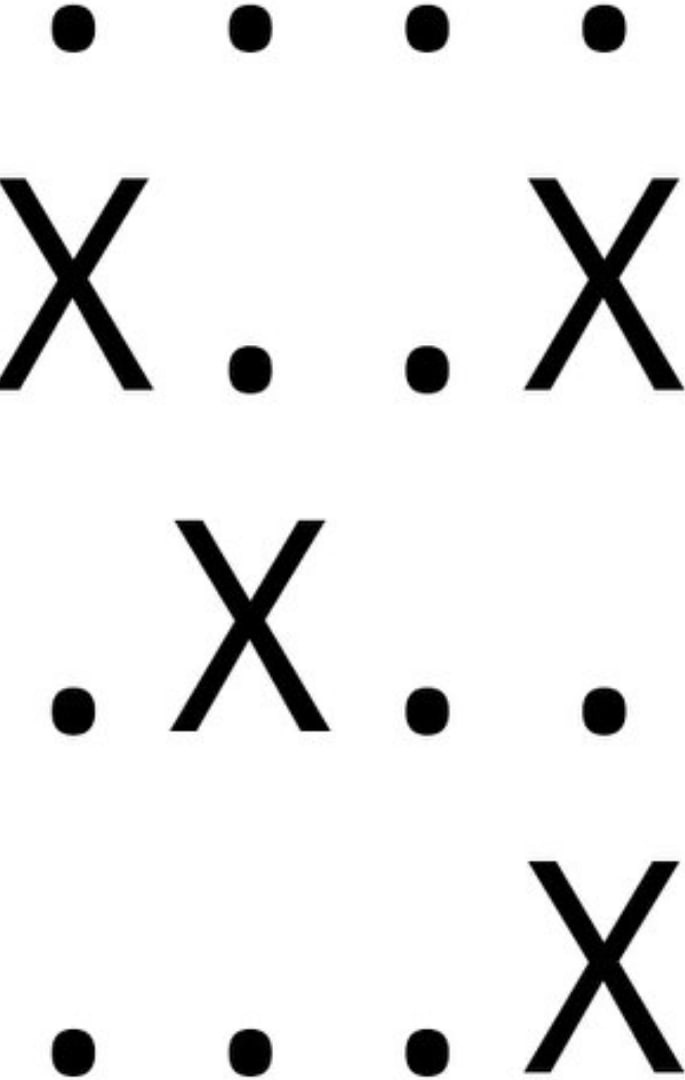
\includegraphics[width=0.15\linewidth]{Source.jpg}
		     \label{fig:my_label}
		 \end{figure}
\end{frame}

\begin{frame}
	\frametitle{Исходные данные} 
		 \begin{block}{}
		     {В следующих четырёх строках дан квадрат с зашифрованным паролем. Все записанные в квадрате символы — строчные и прописные латинские буквы.}
		 \end{block}
		 \begin{figure}
		     \centering
		     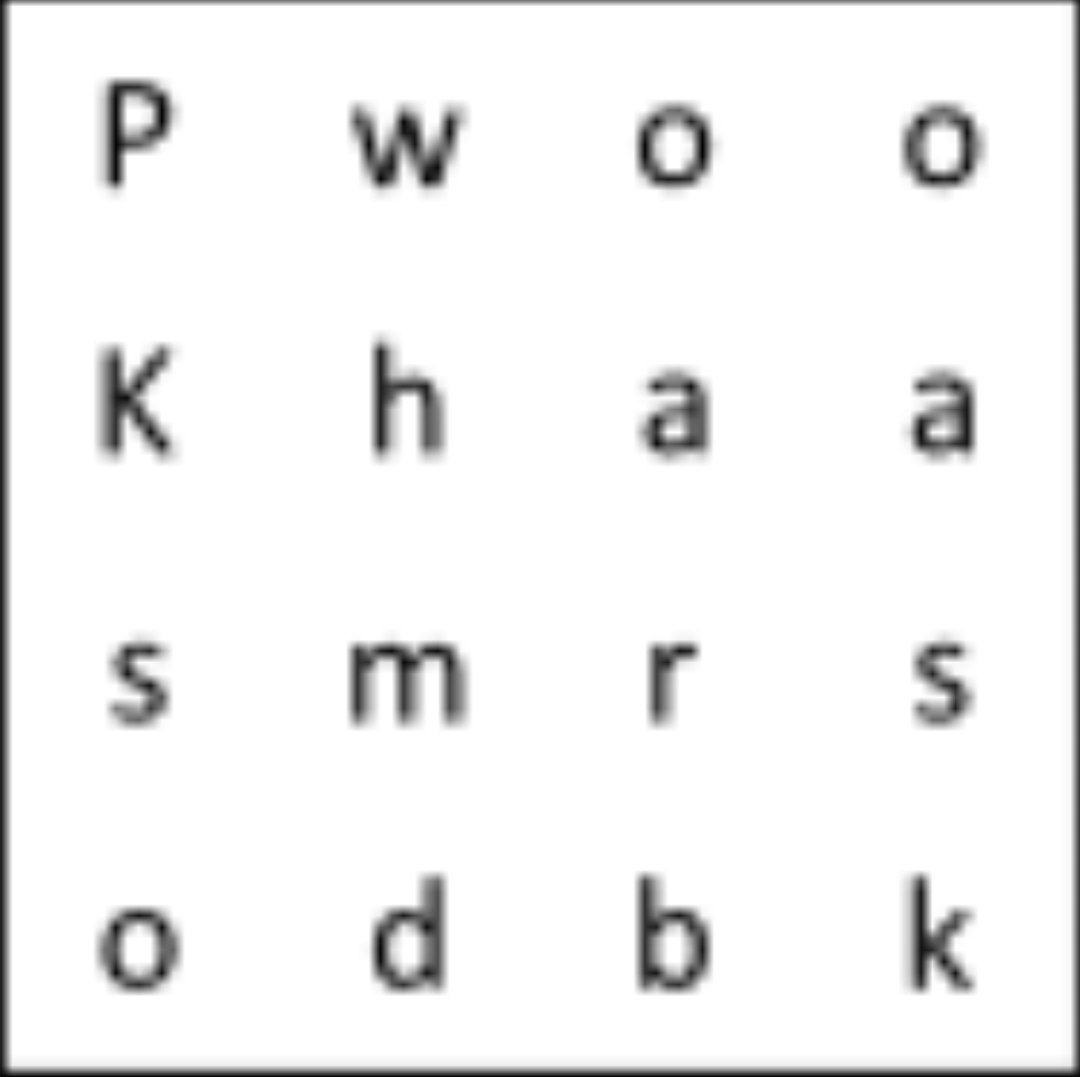
\includegraphics[width=0.3\linewidth]{Result.jpg}
		     \label{fig:my_label}
		 \end{figure}
\end{frame}

\begin{frame}
    \frametitle{Решение}
        \begin{block}{}
		     {Создаётся первый двумерный массив (размером 4x4), состоящий из нулей. Вводим исходные данные первых 4 строк. При обнаружении ячейки с <<Х>> их значения меняются на <<1>>. \\ Создаётся переменная, где будет записан расшифрованный пароль. \\ Создаётся второй двумерный массив (размером 4x4), состоящий из нулей. Вводим исходные данные последних 4 строк. \\ Если в первом массиве находится ячейка с <<1>>, то в строку вводится символ из аналогичной ячейки второго массива. Действие выполняется 4 раза, после чего матрица поворачивается на 90 градусов по часовой стрелке. \\ Действия, описанные в прошлом абзаце, выполняются 4 раза.}
	    \end{block}
\end{frame}

\begin{frame}
	\frametitle{Код}
		\begin{figure}
		     \centering
		     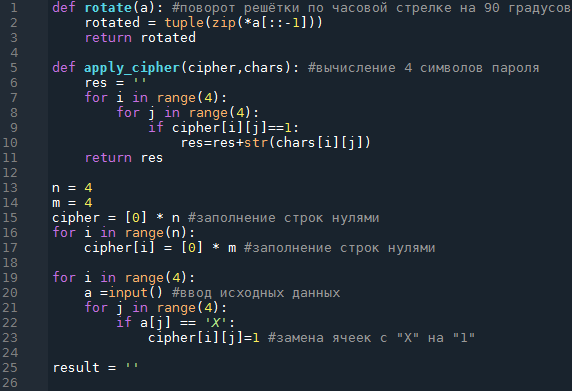
\includegraphics[width=0.9\linewidth]{Screenshot_109.png}
		     \label{fig:my_label}
		 \end{figure}
\end{frame}

\begin{frame}[c]
    \frametitle{Код}
		\begin{figure}
		     \centering
		     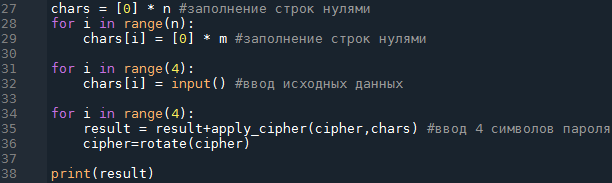
\includegraphics[width=1.0\linewidth]{Screenshot_110.png}
		     \label{fig:my_label}
		 \end{figure}
\end{frame}

\begin{frame}[c]
	\begin{block}{}
    \frametitle{Результат}
		 {В результате работы будет выведена строка, на которой будет изображён ответ:}
	\end{block}
    \begin{itemize}
		\item \textbf{KamkohobPassword}
	\end{itemize}
\end{frame}

\begin{frame}[c]
    \frametitle{Ссылки}
	\begin{itemize}
		\item Код презентации и код задания: \href{https://github.com/QwertyAzerY/KB2-Practice}{https://github.com/QwertyAzerY/KB2-Practice}
	\end{itemize}	
\end{frame}

\frame[plain]{\titlepage}

\end{document}
